\titleSlide{}

\note{\begin{enumerate}
\olditem I always like thos conferences
\olditem where it looks like containers etc are evrywhere
\olditem I like all of that
\olditem but a big part of the world is not that
\olditem I will speak today about the way I work
\olditem and a lot of people still work like that
\olditem IT is not everyones focus
\end{enumerate}}


\frame{%
    \frametitle{user-1000.slice}
    \framesubtitle{Julien Pivotto}
    \begin{itemize}
        \item{Sysadmin at {\inuits{}inuits\small.eu}}
        \item{FLOSS user since 2004}
        \item{systemd user since 2010}
            \begin{itemize}
                \item Exherbo Linux
            \end{itemize}
        \item{DevOps believer}
        \olditem{\textit{\ctr{@roidelapluie}} \ctr{on irc/twitter/github}}
    \end{itemize}
    \note{\begin{enumerate}
    \olditem{FOSS 2004, ubuntu, gentoo, exherbo}
    \olditem{exherbo is a key}
    \olditem{using it (laptop) bef 2010}
    \olditem{systemd mid 2010}
    \olditem{I switched 2010}
    \olditem{collaborative distro}
    \olditem{wrote oct 2010 ovpn unit}
    \olditem{does not mean I know everything}
    \olditem{now I am sysadmin}
    \olditem{in belgium}
\end{enumerate}}
}

\inuitsSlide

\note{\begin{enumerate}
\olditem inuits, open source consultancy
\olditem sysadmin, dev, some SAAS plaform
\olditem be netherlan ukraine cez republic
\olditem more than 50\end{enumerate}}

\picSlide[white]{13932690487_b601b41b32_k.jpg}{https://www.flickr.com/photos/cote/13932690487}{Attribution-2.0}{Introduction}
\note{\begin{enumerate}
\olditem context
\olditem work world
\end{enumerate}}


\begin{iframe}[The DevOps movement]
\item DevOps is a movement born in 2009
\item Collaboration between Developers and Operations
\item Nothing new, just common sense
\item DevOpsDays, a serie of conferences all around the world
\end{iframe}
\note{\begin{enumerate}
\olditem devops movement
\olditem buzz word
\olditem actually something behind
\olditem getting ops and dev to work together
\olditem a community that meet in different places
\olditem solving challenges
\olditem still what is this
\end{enumerate}}

\frame{%
    \frametitle{\#DevOps $\simeq$ C(L)AMS}
    \begin{itemize}
            \LARGE
\item Culture
\item (Lean)
\item Automation
\item Measurement
\item Sharing
    \end{itemize}
\begin{flushright}John Willis and Damon Edwards\end{flushright}
\note{\begin{enumerate}
\olditem DevOps is CLAMS
\olditem Definition from 2010
\olditem it is a cultural and profesionnal
\olditem getting everyone to work together
\olditem reduce time to business
\end{enumerate}}
}

\begin{iframe}[The A of C(L)AMS]
\item Automation reduces human mistakes
\item Continuous Integration/Delivery
\item Reproducable build
\item Reproducable infrastructure
    \olditem {\color{inuits}\ctr{Infrastructure as Code}}
\end{iframe}
\note{\begin{enumerate}
\olditem Automation
\olditem No one touches the server
\olditem Reliability
\olditem Define upfront
\olditem Populate whole environment and know it
\end{enumerate}}

\setbeamercolor{wwh}{fg=yellow,bg=white}
\begin{iframe}[Infrastructure as Code]
\item Automate your infrastructure with code
\item Model your infrastructure
\item Monitoring, security, applications and backups are part of the process
\item Scripts are not IaC
\end{iframe}

\note{\begin{enumerate}
\olditem IAC
\olditem Infra is WRITTEN IN CODE
\olditem infra is a SOFTWARE
\olditem that software contains definitions
\olditem definitions of servers, apps, monit, backup
\olditem this is not bash scripting (more to come)
\olditem ABSTRACTION
\olditem you define system, what is behind should not really matter
\olditem it starts with kickstart
\olditem stays with the whole lifetime of the server
\end{enumerate}}

\begin{iframe}[IaC best practices]
\item Run tests against that code
\item Put it under version control
\item Deploy with CI/CD: dev, uat, prod environments\dots
\end{iframe}
\note{\begin{enumerate}
\olditem How, this is code
\olditem it can be tested
\olditem syntax style
\olditem it can be compiled
\olditem it can be packaged
\olditem Use code best practice
\olditem use the same code for all env
\end{enumerate}}

\begin{frame}[t]
    \frametitle{Configuration Management tools}
    \begin{beamercolorbox}[rounded=true]{wwh}
        \begin{center}
        
\includegraphics[width=2cm]{puppet.png}
        \hspace{0.5cm}
        \hspace{0.5cm}
        
\includegraphics[width=2cm]{chef.png}
        \hspace{0.5cm}
        \hspace{0.5cm}
        
\includegraphics[width=2cm]{ansible.png}
        \\
        
\includegraphics[width=2cm]{saltstack.png}
        \hspace{0.5cm}
        \hspace{0.5cm}
        
\includegraphics[width=2cm]{cfengine.png}
    \end{center}
    \end{beamercolorbox}
\note{\begin{enumerate}
\olditem open source solutions
\olditem first one cfengine
\olditem now puppet/chef/ansible/salt
\olditem i will talk about puppet
\olditem 5 years of puppet xp
\olditem long before systemd reached my pro world
\end{enumerate}}
\end{frame}

\begin{iframe}[Which world is this?]
\item bare-metal
\item virtualization
\item cloud
\item \dots
\note{\begin{enumerate}
\olditem not only containers
\olditem from bare metal to clouds
\olditem can be used in different ways
\olditem a slow world
\olditem traditional IT
\olditem big stateful apps and services
\olditem MOVES SLOWLY (starts el7 since 6 months)
\olditem more machines not more people
\end{enumerate}}
\end{iframe}

\begin{iframe}[Heterogeneous environments]
\item Linux distributions are different
\item Init systems, File hierarchy
\item Even between different releases of the same distro
\item Configuration manegement tools try to abstract that
\end{iframe}
\note{\begin{enumerate}
\olditem most env have mixed distros
\olditem virtualization helps
\olditem thos distros are different
\olditem even between same version
\olditem hence cfgmgmt helps
\olditem abstraction
\end{enumerate}}


\picSlide{systemd-big.png}{}{}{systemd in that picture}
\note{\begin{enumerate}
\olditem in that old world
\olditem at first sight systemd is still coming
\olditem not very integrated
\olditem invisible
\olditem lets dig into it
\olditem found the problems
\end{enumerate}}

\begin{frame}
\frametitle{what people see}
\begin{itemize}
    \item before: distinction between distributions
    \item now: distinction between distributions and systemd or not
    \item tomorrow: it will be hard to provide the all the features of systemd to old distros
\end{itemize}
\end{frame}
\note{\begin{enumerate}
\olditem what people see is this
\olditem before you could change things based in distro
\olditem sometimes need to diff between systemd and not
\olditem people will find how they can use systemd for advanced usage
\olditem will take time
\olditem current status of that world
\olditem one day probably different feature set
\end{enumerate}}

\begin{iframe}[systemd hit majors distros]
\item Reaching Debian Stable and RHEL 7
\item Config management needs to learn it
\item It brings lots of new patterns
\end{iframe}
\note{\begin{enumerate}
\olditem once systemd reaches el7 nothing to be done
\olditem in that world in means 2010 fedora
\olditem expect rhel8 dnf
\olditem a lot of people do not know
\olditem surprised
\olditem afraid
\olditem usual trolls
\end{enumerate}}

\begin{frame}
    \frametitle{Terminology (puppet, simplified)}
\begin{itemize}
    \item resource: description of a small piece (file, service) with desired state
    \item module: collection of resources (e.g.\ a module to setup Mysql)
\end{itemize}
\end{frame}
\note{\begin{enumerate}
\olditem a subset of puppet terminology
\olditem what is needed
\olditem resource file, cron job, nagios definition
\olditem you can get the status
\olditem change that status
\olditem with puppet you describe the desired state
\olditem modules is a collection of that
\olditem abstraction: service optionally tell provider
\olditem bsd debian openbsd openrc runit upstart windows openwrt
\olditem for ex package mysql, config mysql
\end{enumerate}}
\picSlide{service.png}{}{}{Services}
\note{\begin{enumerate}
\olditem services in that world
\olditem lets take a look at traditional vs systemd
\olditem how it does translate
\olditem how it should translate
\end{enumerate}}

\begin{frame}

\frametitle{Services}
\begin{itemize}
    \item Services are basic resources in traditional IT
    \item systemd changes a lot of things in that area
    \item services are now part of the "units" concept
\end{itemize}
\note{\begin{enumerate}
\olditem service, daemon, basic thing
\olditem systemd brings changes
\olditem changes are not always known
\olditem or badly implemented
\end{enumerate}}

\end{frame}
\begin{frame}
\frametitle{Init scripts (without systemd)}
\begin{itemize}
    \item Written from scratch or templates
    \item Different patterns
    \item Sometimes very long, hard to read
\end{itemize}
\note{\begin{enumerate}
\olditem nothing really generic
\olditem standards tries to help
\olditem always a clever guy to write nasty things
\olditem how easy to make typos
\olditem or no/bad indentation
\olditem what is style?
\olditem without talking ordering and so on
\end{enumerate}}
\end{frame}
\begin{frame}
\frametitle{Changing old init scripts}
\begin{itemize}
    \item Why? Solve bugs, ajust niceness, change command\dots
    \item Change the full file!
    \item Template OS and version dependant
\end{itemize}
\note{\begin{enumerate}
\olditem changing is overwriting
\olditem sometimes you need to change the init
\olditem before it was a necessity to fix sometimes bugs
\olditem or make it working like you want
\olditem or x platform
\olditem driving me crazy
\olditem package dependant
\olditem sometimes no init file
\olditem implies bad packaging
\end{enumerate}}
\end{frame}
\begin{frame}
    \frametitle{Ordering (without systemd)}
    \begin{center}
        
\includegraphics[height=.6\paperheight]{pcs.png}
    \end{center}
\note{\begin{enumerate}
\olditem very high level view
\olditem inside a module
\olditem arrows are dependencies
\olditem strong implication
\olditem same tool who updates
\olditem package put the new file
\olditem overwrite again
\olditem CONDRESTART? problem coz overwrite your init script
\end{enumerate}}
\end{frame}
\begin{iframe}[Unit files (with systemd)]
\item ini-like syntax
\item Self-explanatory
\item Standardized accross distros
\note{\begin{enumerate}
\olditem any tool can atomically edit ini
\olditem YOu change because it adds value
\olditem or replace it
\olditem easy to launch a daemon
\olditem majority cross distro
\olditem clear syntax
\olditem really easy to read
\olditem systemctl cat
\end{enumerate}}
\end{iframe}

\begin{frame}
    \begin{center}
        \huge
        Here is the rule:\\
        Packaged files go in /lib.
        Config management tools override in /etc.
    \end{center}
\note{\begin{enumerate}
\olditem systemd rule
\olditem /etc overwirte the rest
\olditem /etc for the sysadmin
\olditem he does not touch server, remember
\olditem so sysadmin is puppet
\olditem modules can just write in /etc
\olditem people do not know
\olditem use old pattern with same problem
\olditem systemd is not an improvement for them
\end{enumerate}}
\end{frame}

\begin{iframe}[No conflict with vendor files]
\item Can be overriden in /etc/systemd/system
\item Not afraid of package updates
\item Partial override possible
\end{iframe}
\note{\begin{enumerate}
\olditem this method is relevant
\olditem avoid packages to use /etc
\olditem good for condrestart and so on
\olditem partial override are cool
\end{enumerate}}


\begin{frame}[fragile]
    \frametitle{Partial override example}
    \center{\large/etc/systemd/system/httpd.service.d/niceness.conf}
\lstset{basicstyle=\large\fsfont}
\begin{lstlisting}
               [Service]
               Nice=3
\end{lstlisting}
\note{\begin{enumerate}
\olditem how complex was this before
\olditem if you want this on diff env
\olditem diff httpd release
\olditem just one or multiple property
\olditem systemctl cat
\olditem niceness is a basic example
\olditem change start command, add dependencies
\end{enumerate}}
\end{frame}


\begin{frame}{The surprise}
    \begin{itemize}
\item Creating the file is not enough
\item systemctl daemon-reload
\end{itemize}
\texttt{Notice: /Service[mariadb]/ensure: ensure changed {}'stopped' to {}'running'}
\note{\begin{enumerate}
\olditem that comes as a surprise for many people
\olditem confmgmt tool does not show wny warning
\olditem puppet does not do anything
\olditem yesterday davids talk showed that this is costful
\olditem chose the right pattern to do that
\olditem systemctl cat
\olditem systemctl-delta
\olditem not possible to reload one unit
\end{enumerate}}
\end{frame}
\begin{frame}
    \frametitle{Ordering (with systemd)}
    \begin{center}
        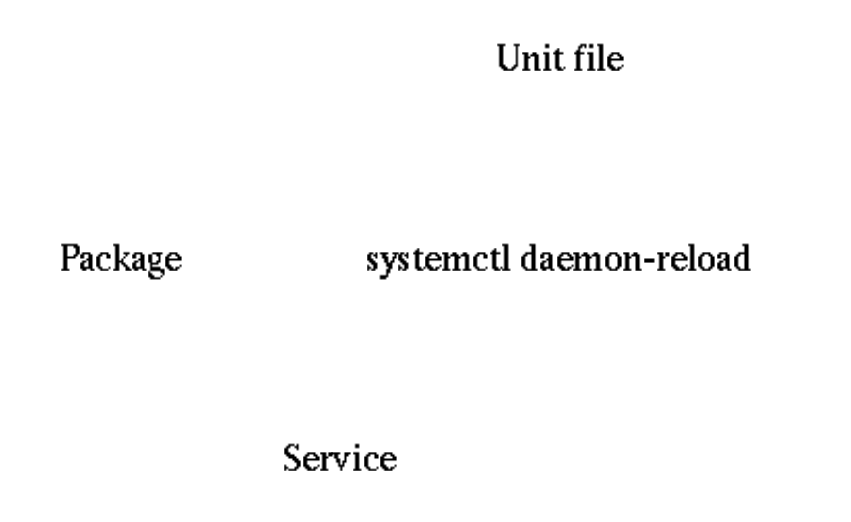
\includegraphics[height=.6\paperheight]{unit.png}
    \end{center}
\note{\begin{enumerate}
\olditem this is now: you know need to add that command
\olditem dependency
\olditem no dep against package
\olditem dependency at the service level
\olditem condrestart might imply another dependency
\end{enumerate}}
\end{frame}
\begin{frame}\frametitle{daemon-reload in Puppet}
    \lstinputlisting{systemctl-reload.pp}

\note{\begin{enumerate}
\olditem look we define state (content, status)
\olditem how it is done in puppet
\olditem only if file changed
\olditem change is also creation
\olditem if command of file fails service wont start
\end{enumerate}}
\end{frame}

\begin{frame}
    \frametitle{systemctl daemon-reload}
    \begin{center}
        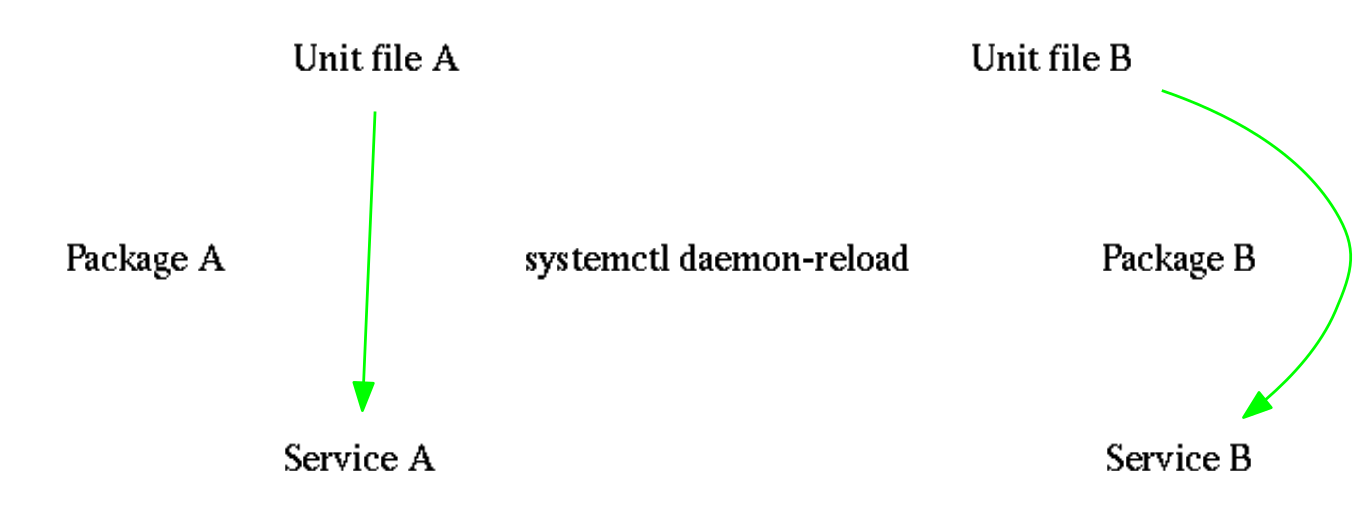
\includegraphics[width=.9\paperwidth]{trap.png}
    \end{center}
\note{\begin{enumerate}
\olditem when you have multiple time
\olditem want to call one
\olditem lazyness
\olditem SPOF
\olditem services wil start at approx same time
\olditem if one file fails (templating error)
\olditem nothing will start or restart
\olditem notify between file and service
\olditem not command and service (restart all serv all the time)
\olditem file change, service restart
\olditem file change, service no restart NO ROLLBACK
\olditem service runs the old parameters
\end{enumerate}}
\end{frame}

\begin{frame}
    \frametitle{systemctl daemon-reload}
    \begin{center}
        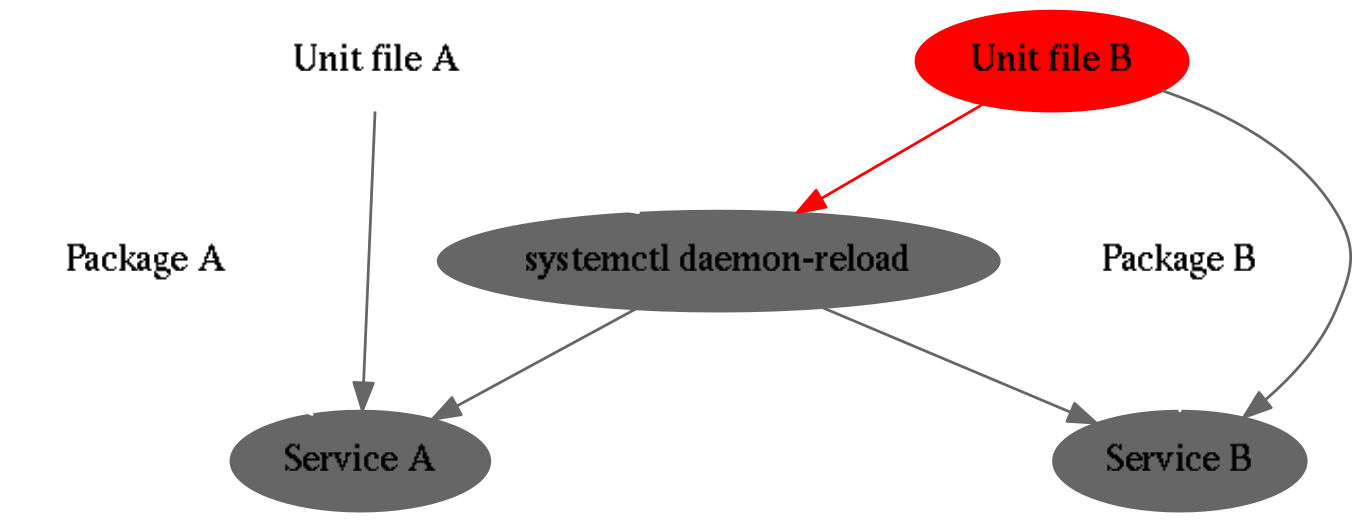
\includegraphics[width=.9\paperwidth]{trap2.png}
    \end{center}
\note{\begin{enumerate}
\olditem when you have multiple time
\olditem want to call one
\olditem lazyness
\olditem SPOF
\olditem services wil start at approx same time
\olditem if one file fails (templating error)
\olditem nothing will start or restart
\olditem notify between file and service
\olditem not command and service (restart all serv all the time)
\olditem file change, service restart
\olditem file change, service no restart NO ROLLBACK
\olditem service runs the old parameters
\end{enumerate}}
\end{frame}

\begin{frame}
    \frametitle{systemctl daemon-reload}
    \begin{center}
        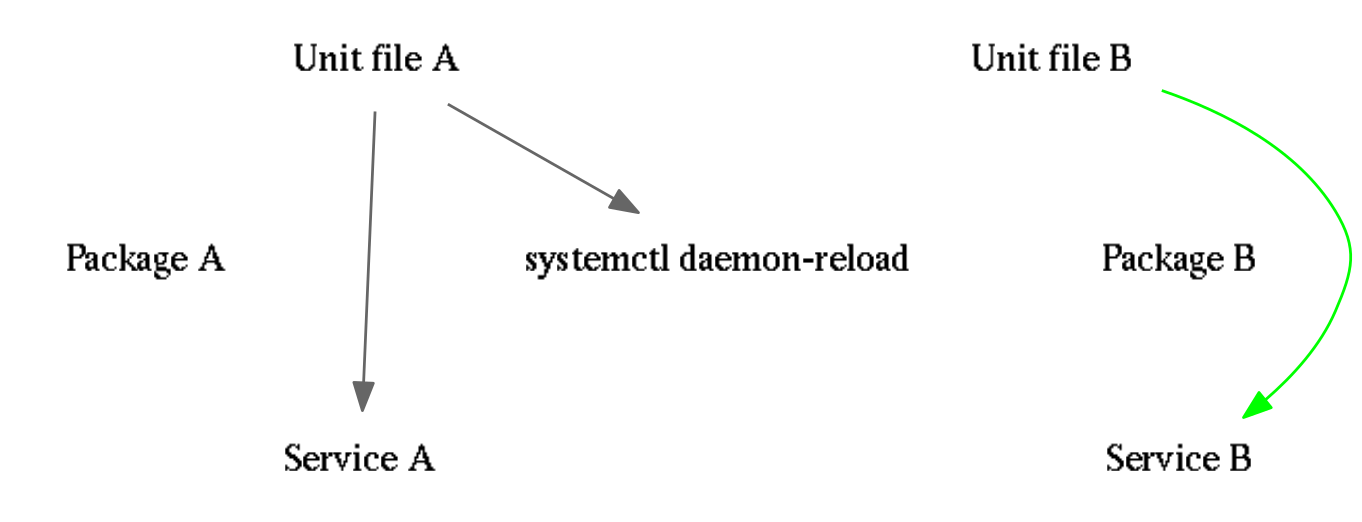
\includegraphics[width=.9\paperwidth]{trap4.png}
    \end{center}
\note{\begin{enumerate}
\olditem when you have multiple time
\olditem want to call one
\olditem lazyness
\olditem SPOF
\olditem services wil start at approx same time
\olditem if one file fails (templating error)
\olditem nothing will start or restart
\olditem notify between file and service
\olditem not command and service (restart all serv all the time)
\olditem file change, service restart
\olditem file change, service no restart NO ROLLBACK
\olditem service runs the old parameters
\end{enumerate}}
\end{frame}


\begin{frame}
    \frametitle{systemctl daemon-reload ordering}
    \begin{center}
        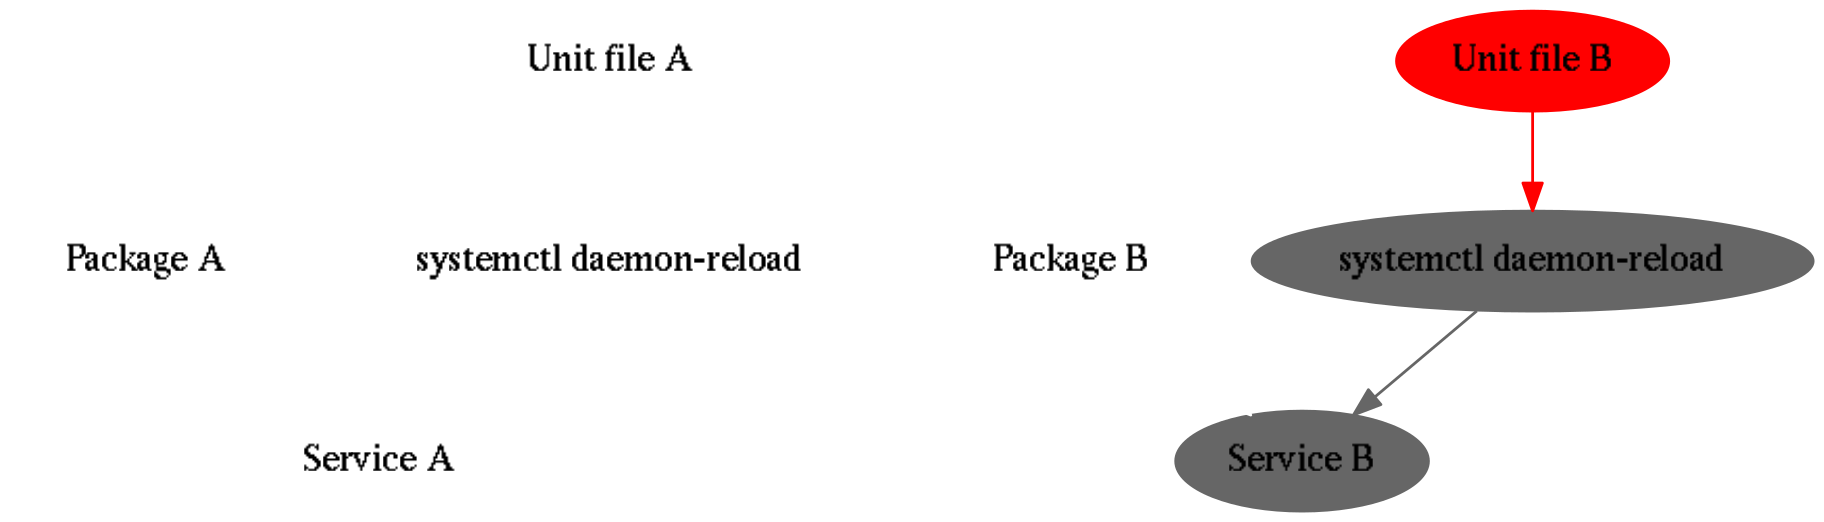
\includegraphics[width=.9\paperwidth]{trap3.png}
    \end{center}
\note{\begin{enumerate}
\olditem one service one call
\olditem file trigger command triggers service
\olditem we indeed need to atomically update this
\olditem no really any best solution at the moment
\olditem new pattern that we need to be used to
\olditem hopefulle systemctl will not exit with non 0
\olditem but service will fail to start
\olditem so we will notice
\end{enumerate}}
\end{frame}


\begin{iframe}[Prevent a service to start]
\item Classic init allows to disable services
\item Configmgmt tools do not care
\item chmod 000 /etc/init.d/mysqld
\end{iframe}
\note{\begin{enumerate}
\olditem if you do not want a service to start
\olditem rememeber puppet is the sysadmin
\olditem he will launch the script
\olditem hack hack hack
\olditem remove file
\olditem change mode
\olditem bad because alter package content
\olditem (ONCE AGAIN)
\olditem very bad
\end{enumerate}}

\begin{iframe}[Masking services]
\item ln -s /dev/null /etc/systemd/system/mysqld.service
\item systemctl daemon-reload
\item Done. It can't be started anymore
\end{iframe}
\note{\begin{enumerate}
\olditem even more important to disable a seice with systemd
\olditem implicit starts: deps, targets, timers
\olditem MASKING to the rescue
\olditem systemctl mask
\olditem zero file or /dev/null
\olditem needs systemctl daemon reload
\olditem you can STOP a maked service
\end{enumerate}}
\begin{frame}\frametitle{masking in Puppet}
    \lstinputlisting{mask.pp}

\note{\begin{enumerate}
\olditem simple way to create the file
\olditem not to forget to stop the service
\olditem not to forget the daemon reload
\end{enumerate}}
\end{frame}


\picSlide[white]{3748310435_c321366fe4_b.jpg}{https://www.flickr.com/photos/brightmeadow/3748310435}{Attribution-ShareAlike 2.0}{(tmp) files}
\note{\begin{enumerate}
\olditem second topic tmp files
\olditem another way where systemd brings unification
\end{enumerate}}

\begin{frame}\frametitle{tmpfiles before systemd}
\begin{center}Several techniques: tmpfs, tmpwatch\end{center}
    \lstinputlisting{tmpwatch}


\note{\begin{enumerate}
\olditem complex code for handling special case
\olditem distro specific
\olditem not a list
\olditem packaged so you do not want to change
\olditem but sometimes you need
\olditem non obvious
\end{enumerate}}
\end{frame}

\begin{frame}\frametitle{tmpfiles with systemd}
\begin{center}systemd-tmpfiles\end{center}
    \lstinputlisting{systemd-tmpfiles}

\note{\begin{enumerate}
\olditem DAMNED THIS IS TEXT
\olditem no wrappers
\olditem clear doc (do not need every day)
\olditem ediatble by cfgmgmt tools
\olditem wait for it.. remember /lib stuff?
\end{enumerate}}
\end{frame}
\begin{frame}\frametitle{tmpfiles with systemd}
\begin{itemize}
    \item Again, simple text files
    \item Can be overwritten in /etc
    \item Yet another command to launch
    \end{itemize}
\note{\begin{enumerate}
\olditem cool /etc trick works AGAIN
\olditem no ned to overwrite packge/distro file
\olditem again fi you do the ackaging change /lib/tmpfiles
\olditem puppet is the sysadmin that wite files
\olditem need some commands to be takin in cosideration
\end{enumerate}}
\end{frame}
\begin{frame}\frametitle{tmpfiles with systemd and Puppet}
    \lstinputlisting{systemd-tmpfiles-puppet}
\note{\begin{enumerate}
\olditem again ideally one command per file
\olditem more dependencies
\olditem more fun
\olditem quite of the downside
\olditem not only create, edge cases possibles
\end{enumerate}}
\end{frame}

\picSlide[white]{15110111516_aea024b9df_o.jpg}{https://www.flickr.com/photos/southbeachcars/15110111516}{Attribution 2.0}{Timers}

\begin{frame}\frametitle{Traditional cron}
    \lstinputlisting{cron}\pause
    \LARGE 30 times.
\end{frame}
\note{\begin{enumerate}
\olditem agin that is native
\olditem how easy is this? not
\olditem hwo fun is this? not
\olditem real world simplified example
\end{enumerate}}
\begin{iframe}[What's wrong?]
\item No one reads those mails
\item Do not keep track of exit code
\item Hard to read that crontab
\item How to reproduce the script?
\end{iframe}
\note{\begin{enumerate}
\olditem when does it fail
\olditem why
\olditem efter we see we redirected output to dev null
\olditem EFFECTIVELY REMOVING STDERR to not be spammed
\olditem appens all the time
\end{enumerate}}

\begin{iframe}[The systemd approach: timers]
\item Describe the job in a service file
\item Add a timer file
\item Enable/start the timer service
\end{iframe}
\note{\begin{enumerate}
\olditem one could use systemd run, env files
\olditem that would be HALF the systemd approach
\olditem I will show the EFFECTIVE systemd way
\olditem it is called timers
\olditem it requires more work
\olditem enable timer instead of service
\olditem write timer and service
\olditem easy to package
\end{enumerate}}

\begin{iframe}[Why is it better?]
\item Easy to reproduce (launch the service unit)
\item Logs go to the journal, isolated by unit
\item All the advantages of systemd units
\end{iframe}
\note{\begin{enumerate}
\olditem cross distro
\olditem NEED INDEMPOTANT services
\olditem do not need to send the logs to everyont
\olditem icinga check status of service
\olditem journald logs all the things
\olditem centralize the logs
\olditem logstash cat emails, journald
\olditem all the adv and downsides of systemd units
\end{enumerate}}

%INTERFACES
\picSlide[white]{4391670988_dabdecaa55_o.jpg}{https://www.flickr.com/photos/clonedmilkmen/4391670988}{Attribution-ShareAlike 2.0}{Networking}
\note{\begin{enumerate}
\olditem quickly talking about interface names
\olditem explicitely put PHYSUCAL network photograph
\olditem private cloud, baremetal, vms
\end{enumerate}}
\begin{iframe}[Networking]
\item New name interfaces
\item Makes sense because it is reliable
\item Does not really meet configmgmt requirements
\end{iframe}
\note{\begin{enumerate}
\olditem one slide, this is wip
\olditem new networking interfacename kind of make sense
\olditem hard on multiple hardware (I am pragmatic)
\olditem we never have completely the same hardware
\olditem we need to enable firewall rules for example
\olditem hard to define the same of all infra
\olditem hard to know upfront
\end{enumerate}}

\picSlide{systemd-big.png}{}{}{Conclusion}
\note{\begin{enumerate}
\olditem brings me to the conclusion
\olditem the added value of BRAND NEW systemd
\olditem CAN WE FOCUS ON TECHNICAL STUFF
\olditem Yes now its there WE CAN
\end{enumerate}}

\begin{iframe}[systemd is complex\dots]
\item It drags in a bunch of new pattern
\item It supports a lot of scenarios
\item It can do really advanced things
\end{iframe}
\note{\begin{enumerate}
\olditem YES systemd is complete
\olditem YES systemd is feature complete
\olditem YES systemd changes a lot of things
\olditem YES you can DO A LOT with systemd natively
\olditem YES those are not ONLY bash scripts
\end{enumerate}}

\begin{iframe}[\dots but based on simple bricks]
\item Ini-like file format
\item Easy to read, to change
\item Config management tools have all the base bricks to manage that
\end{iframe}
\note{\begin{enumerate}
\olditem NO Init files are not complex
\olditem YES any cfgmgmt tool can drop those file
\olditem Even atomically update
\olditem Partial overrides are awesome: no need to change base modules
\olditem config tools have the base bricks
\end{enumerate}}

\begin{iframe}[There are surprises]
\item systemctl daemon-reload
\item systemd-tmpfiles
\item timers
\end{iframe}
\note{\begin{enumerate}
\olditem YES THERE ARE THINGS TO LEARN
\olditem it you do not LIKE TO LERAN what is your job
\olditem this world evolves slowly
\olditem lots of testing, waiting, take the time
\olditem DO NOT APPLY blindly the same patterns
\end{enumerate}}

\begin{iframe}[You need to know the rules]
\item Take time to learn how this works
\item There is a gap between systemd devs and sysadmins
\item There are new non-obvious patterns for sysadmins
\item But at the end eveyone can win
\end{iframe}
\note{\begin{enumerate}
\olditem IF YOU KNOW THE SYSTEMD RULES
\olditem Help other
\olditem S of devops is sharing
\olditem improve the modules
\olditem embrace change
\olditem CLOSE THE GAP
\olditem as sysadmin you can not ignore systemd
\end{enumerate}}

\begin{iframe}[The tools side]
\item The tools natively supports systemd services
\item Chef goes a lot further
\item https://github.com/nathwill/chef-systemd
\end{iframe}
\note{\begin{enumerate}
\olditem Integration is poor in Puppet
\olditem partly because they support many systems
\olditem use case example: systemd-run
\olditem looks like more work has been done in chef
\olditem ONLY SERVICES
\olditem things to improve
\olditem keeping the same practices
\olditem modeling, IAC, etc
\end{enumerate}}

\begin{iframe}[A Story of gaps]
\olditem Gap between systemd and configmgmt tools
\olditem Gap between systemd community and cfgmgmt tools community
\olditem Together we can close those gaps
\end{iframe}
% services

% timers

% 


\CenterSlide{Any Question?}

\contactSlide

